%%%%%%%%%%%%%%%%%%%%%%%%%%%%%%%%%%%%%%%%%%%%%%%%%%%%%%%%%%%%%%%%%%%%%%%%%%
%%%%%% Ajit Kumar Sahoo, School of Computer and Information Sciences,
%%%%%% University of Hyderabad, Hyderabad, India-500046
%%%%%% Email: sahooajitkumar85@gmail.com
%%%%%% https://ajitsahoocs.github.io/
%%%%%%%%%%%%%%%%%%%%%%%%%%%%%%%%%%%%%%%%%%%%%%%%%%%%%%%%%%%%%%%%%%%%%%%%%%%
\documentclass{beamer}
\hypersetup{pdfpagemode=FullScreen} %full screen mode
\setbeamertemplate{navigation symbols}{}
\usepackage[english]{babel} %designed for typesetting lebels(addr lebel,sticky lebels,etc)
\usepackage[utf8]{inputenc} %Accept different input encodings
\usepackage{amsmath,amssymb} 
\usepackage[T1]{fontenc} %for font encoding
\usepackage{times} % use times font instead of default
\usepackage{curves} %for drawing curves
\usepackage{verbatim} %paragraph making environment 
\usepackage{multimedia} %for multimedia like animation,movie etc...
\usepackage{mathptmx} % font style
\usepackage{graphicx} % Allows including images
\usepackage{booktabs} % Allows the use of \toprule, \midrule and \bottomrule in tables
\usepackage{hyperref}
\usepackage{xcolor}
\usepackage{import}


\newcommand{\incfig}[2][1]{%
    \def\svgwidth{#1\columnwidth}
    \import{./figures/}{#2.pdf_tex}
}

\usepackage{algorithm,algorithmic}
\renewcommand{\algorithmicrequire}{\textbf{Input:}}
\renewcommand{\algorithmicensure}{\textbf{Output:}}
\usepackage{lipsum}
\setbeamertemplate{caption}[numbered] % For numbering figures



\mode<presentation> {

% The Beamer class comes with a number of default slide themes
% which change the colors and layouts of slides. Below this is a list
% of all the themes, uncomment each in turn to see what they look like.

%\usetheme{default}
%\usetheme{AnnArbor}
%\usetheme{Antibes}
%\usetheme{Bergen}
%\usetheme{Berkeley}
%\usetheme{Berlin}
%\usetheme{Boadilla}
%\usetheme{CambridgeUS}
%\usetheme{Copenhagen}
%\usetheme{Darmstadt}
%\usetheme{Dresden}
%\usetheme{Frankfurt}
%\usetheme{Goettingen}
%\usetheme{Hannover}
%\usetheme{Ilmenau}
%\usetheme{JuanLesPins}
%\usetheme{Luebeck}
\usetheme{Madrid}
%\usetheme{Malmoe}
%\usetheme{Marburg}
%\usetheme{Montpellier}
%\usetheme{PaloAlto}
%\usetheme{Pittsburgh}
%\usetheme{Rochester}
%\usetheme{Singapore}
%\usetheme{Szeged}
%\usetheme{Warsaw}

% As well as themes, the Beamer class has a number of color themes
% for any slide theme. Uncomment each of these in turn to see how it
% changes the colors of your current slide theme.

%\usecolortheme{albatross}
%\usecolortheme{beaver}%this one also
%\usecolortheme{beetle}
%\usecolortheme{crane} % also use this one
%\usecolortheme{dolphin}
%\usecolortheme{dove}
%\usecolortheme{fly}
%\usecolortheme{lily}
%\usecolortheme{orchid}
%\usecolortheme{rose}
%\usecolortheme{seagull}
%\usecolortheme{seahorse}
\usecolortheme{whale} % Best one
%\usecolortheme{wolverine} %use can use this also

%\setbeamertemplate{footline} % To remove the footer line in all slides uncomment this line
%\setbeamertemplate{footline}[page number] % To replace the footer line in all slides with a simple slide count uncomment this line

%\setbeamertemplate{navigation symbols}{} % To remove the navigation symbols from the bottom of all slides uncomment this line
}

\usepackage{graphicx} % Allows including images
\usepackage{booktabs} % Allows the use of \toprule, \midrule and \bottomrule in tables
\setbeamercovered{transparent}
\setbeamertemplate{bibliography item}[text]
\setbeamertemplate{theorems}[numbered]
\setbeamerfont{title}{size=\Large}%\miniscule,command,tiny, scriptsize,footnotesize,small,normalsize,large,Large,LARGE,huge,Huge,HUGE
\setbeamerfont{date}{size=\tiny}%{\fontsize{40}{48} \selectfont Text}

\setbeamertemplate{itemize items}[ball] % if you want a ball
\setbeamertemplate{itemize subitem}[circle] % if you wnat a circle
\setbeamertemplate{itemize subsubitem}[triangle] % if you want a triangle


%------------------customized frame----------------------------
\newcounter{cont}

\makeatletter
%allowframebreaks numbering in the title
\setbeamertemplate{frametitle continuation}{%
   % \setcounter{cont}{\beamer@endpageofframe}%
    %\addtocounter{cont}{1}%
   % \addtocounter{cont}{-\beamer@startpageofframe}%
   % (\insertcontinuationcount/\arabic{cont})%
}
\makeatother
%-----------------------customized-----------------------------




%----------------------------------------------------------------------------------------
%	TITLE PAGE
%----------------------------------------------------------------------------------------

\title[Non-Flat universe BAO]{Baryon acoustic oscillations in a non-flat universe} % The short title appears at the bottom of every slide, the full title is only on the title page

%\author[AKS]{Ajit Kumar Sahoo \texorpdfstring{\scriptsize Regd No: 16MCPC03}{}}
\author[SSW]{\texorpdfstring{Santiago Sanz Wuhl}{Author}}

\institute[UCO] % Your institution as it will appear on the bottom of every slide, may be shorthand to save space
{

{\small Trabajo de Fin de Grado}\\
\medskip
{Código FS22-17-FSC}\\
\begin{center}

\includegraphics[width=0.2\textwidth]{uoh.png}
\end{center}
\medskip
{\normalsize Grado de Física}\\
Facultad de Ciencias \\
Universidad de C\'ordoba

%\medskip
%\textit{john@smith.com} % Your email address
}
%This will place the image at position "30 right/left and 120 up/down" relative to the top left corner of the current page.
%\titlegraphic{%
%  \begin{picture}(0,0)
%    \put(30,125){\makebox(0,0)[rt]{
\includegraphics[width=2.5cm]{uoh.png}}}
%  \end{picture}}
 \date{\today} % Date, can be changed to a custom date
\begin{document}

\begin{frame}
\titlepage % Print the title page as the first slide
\end{frame}
\begin{frame}
  \frametitle{Contents}
 % \tableofcontents[pausesections,shaded]
 \tableofcontents
\end{frame}
% TABLE OF CONTENTS AT BEGIN OF EACH SECTION
\AtBeginSection[]{
  \begin{frame}<beamer>
    \frametitle{Current Section}
   \tableofcontents[currentsection]
  \end{frame}}
%----------------------------------------------------------------------------------------
%	PRESENTATION SLIDES
%----------------------------------------------------------------------------------------


%-------------------------------------------------------------------------------
%-------------------------------INTRODUCTION--------------------------------
%-----------------------------------------------------------


\section{Resumen} 
\begin{frame}[allowframebreaks]
\frametitle{Resumen}

\quad En este trabajo de fin de grado se hace uso de herramientas de computaci\'on de alto rendimiento y an\'alisis de datos para estudiar los efectos de ligeras variaciones en el \textbf{modelo cosmol\'ogico est\'andar} $\Lambda$CDM. Este modelo asume un universo \textbf{espacialmente plano}, si bien las observaciones son compatibles con una curvatura no nula.\\
\vspace{0.2cm}
\quad Este trabajo se basa en las \textbf{oscilaciones} \textbf{acústicas} \textbf{de} \textbf{bariones}, un fen\'omeno que nos permite estudiar el comportamiento del universo en sus etapas m\'as tempranas. \\

\vspace{0.2cm}
\quad Después de analizar el catálogo de galaxias del cartografiado \textbf{eBOSS}, obtenemos los siguientes resultados: $D_H/r_d = 18.66\pm 0.72$ y $D_M/r_d = 18.28\pm 0.53$ para un universo plano, en concordancia con los resultados para otros valores no nulos del \textbf{parámetro} \textbf{de} \textbf{curvatura} $\Omega_k$, y lo que es m\'as importante, con resultados anteriores en el campo.
\end{frame}

\section{Introduction}
\begin{frame}[allowframebreaks]
\frametitle{The Baryon Acoustic Oscillations}

\begin{enumerate}
  \item \textbf{Early Universe}: Primordial density perturbations are created due to quantum fluctuations during inflation.
  
  \item \textbf{Primordial plasma}:  The high temperatures keep the universe ionized, tightly binding photons and baryons.
  
  \item \textbf{Acoustic Oscillations}: Perturbations in the equilibrium between gravitational attraction and thermal radiation pressure cause pure acoustic waves to propagate through the plasma (BAO).
  
  \item \textbf{Recombination}: As the universe expands and cools, the Thomson Scattering mechanism stops being effective and photons decouple from the plasma, `turning off' the interaction and freezing the Acoustic Waves.
  
  
\end{enumerate}

\end{frame}
\begin{frame}[allowframebreaks]
\frametitle{The Baryon Acoustic Oscillations}
\begin{figure}[b]
	\centering
	\subfigure{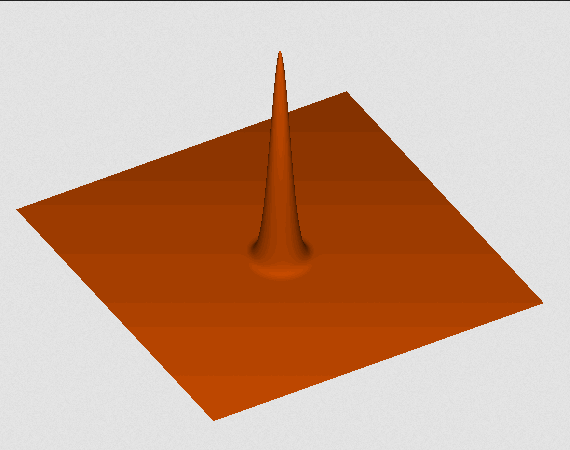
\includegraphics[width=0.3\textwidth]{baogif1.png}}
	\subfigure{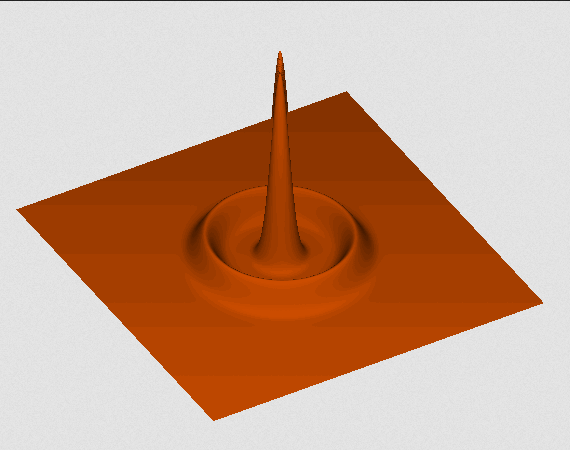
\includegraphics[width=0.3\textwidth]{baogif2.png}}
	\subfigure{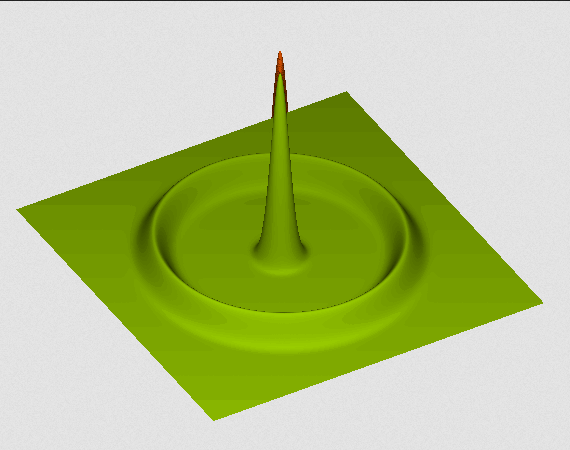
\includegraphics[width=0.3\textwidth]{baogif3.png}}
	\caption{Different time evolution stages of the Baryon Acoustic Oscillations}
\end{figure}

\end{frame}

\begin{frame}[allowframebreaks]
\frametitle{The BAO analysis}
Considering the distribution of the distances at which two galaxies are found of one another, we finde the correlation function $\xi(r)$ and its Fourier Transform, the power spectrum $P(k)$.
\begin{figure}[b] \centering
	\subfigure{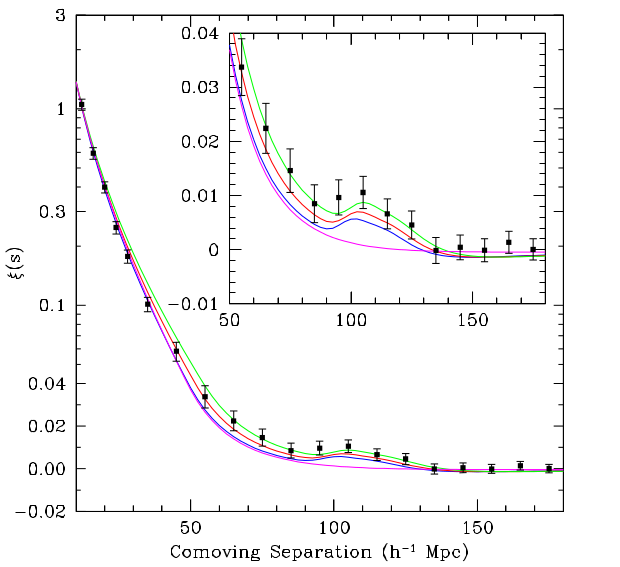
\includegraphics[width=0.3\textwidth]{../figs/sdss_xi.png} \label{fig:sdss}}
	\hspace{0.2pt}
	\subfigure{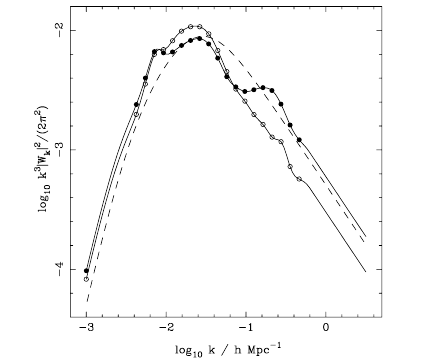
\includegraphics[width=0.32\textwidth]{../figs/2df_pk.png}	\label{fig:2df}}
	\caption{First BAO observations by the SDSS and the 2dF collaborations\\ \centering \textbf{Note} the local maxima at $s=r_d$ and $k=2\pi /r_d$.}
	\label{fig:2005-results}
\end{figure}
\end{frame}


\begin{frame}[allowframebreaks]
\frametitle{The $\Lambda$CDM model}
\begin{table}[t]
\begin{center}
\begin{tabular}{|c|c|c|}
\hline
\textbf{Parameter} & \textbf{Parameter} \textbf{Name} & \textbf{Fiducial} \textbf{Value} \\
\hline
$\Omega_b$ & Baryon Density Parameter & 0.0481 \\
$\Omega_c$ & Dark Matter Density Parameter & 0.2604 \\
$H_0$ & Hubble Constant & 67.6 kms$^{-1}$Mpc$ ^{-1}$ \\
$\tau_{\text{reio}}$ & Reionization Optical Depth & 0.09 \\
$A_s$ & Scalar Perturbation Amplitude & 2.0403 × 10$^{-9}$ \\
$n_s$ & Scalar Spectral Index & 0.97 \\
\hline
$\Omega_k$ & Curvature Parameter & $[-0.20, 0.20]$ \\
\hline
\hline
$r_d$ & Sound Horizon at Recombination & 147.784 Mpc \\
$D_H/r_d$ & Hubble distance & 18.7 \\
$D_M/r_d$ & Angular diamater distance& 18.3 \\
$\Omega_\Lambda$ & Dark Energy Density Parameter& [0.49, 0.89] \\
$\Omega_m$ & Matter Density Parameter & 0.31 \\
\hline
\end{tabular}
\end{center}
\label{tab:fid-values}
\end{table}
\end{frame}




%-------------------------------------------------------------------------------------------------------------------------------
\section{Objectives}
\begin{frame}[allowframebreaks]
\frametitle{Objectives}
\begin{enumerate}
  \item Review the theoretical background of \textbf{BAO} \textbf{observables}: physical origin, mathematical formulation, and become familiar with the software tools for data analysis and visualization.
  %\item Learn to use these \textbf{software} \textbf{tools} for data preprocessing, analysis, and visualization of BAO-related cosmological data sets.
  \item Investigate the impact of \textbf{different} \textbf{values} \textbf{of} \textbf{the} \textbf{curvature} \textbf{parameter} $\Omega_k$ on the behavior of BAO observables.
  \item Analyze the most recent observational data on BAO observables, obtained from the \textbf{eBOSS} \textbf{experiment}, and compare the results with theoretical predictions for different values of $\Omega_k$.
	\item Make use of \textbf{high} \textbf{performance} \textbf{computing} to solve Physics problems.
  %\item Specific \textbf{data} \textbf{analysis} software development.
  \item Learn to \textbf{remotely} control computer clusters via \textbf{SSH} (Secure Shell).
\end{enumerate}
\end{frame}

\section{Materials and methods}
\begin{frame}[allowframebreaks]
\frametitle{Mathematics, software and hardware}

\begin{enumerate}
	\item \textbf{Mathematics} The Fast Fourier Transform algorithm
	\item \textbf{Software}
		\begin{itemize}
			\item \textbf{RUSTICO} Measures the power spectrum of a given galaxy catalog\footnote{In our case, the Luminous Red Galaxies of the extended Baryon Oscillation Spectroscopy Survey (LRG eBOSS)} as the Fourier Transform of the correlation function
			\begin{align}
				\xi(\textbf{r}) = \left<\delta(\textbf{x})\delta (\textbf{x}') \right>,\, \text{with}\, \delta(\textbf{x}) = \frac{\rho(\textbf{x}) - \overline{\rho}}{\overline{\rho}}
			\end{align}
		\item \textbf{CLASS} The theoretical power spectrum for a given cosmology.
		\item \textbf{BRASS} Returns the best-fit parameters in the line-of-sight ($\alpha_\parallel$) and in the transverse ($\alpha_\perp$) direction  of the theoretical power spectrum to the measured one, along with their standard deviations.
		\end{itemize}
	\item \textbf{Hardware} The clusters from the \textit{FQM-378} research group in the Universidad de Córdoba.

\end{enumerate}


\end{frame}

\begin{frame}{Pipeline}

	\begin{figure}[h]
		\centering
		\incfig{pipeline}
		\caption{The pipeline used to measure the desired cosmological distances}
		\label{fig:-figs-pipeline-pdf}
	\end{figure}
\end{frame}

\section{Results}
\begin{frame}{Procedure}

Using the mentioned pipeline, we followed the following procedure to obtain the desired results
\begin{itemize}
	\item A single \textbf{fixed flat cosmology} template is generated using CLASS
	\item For $\Omega_k$ in the range $\left[ -0.20, 0.20 \right] $ in steps of $0.05$, nine different power spectrums are \textbf{measured} from the eBOSS galaxy catalog.
	\item Using BRASS, we fit the template to \textbf{each power spectrum}, obtaining $\alpha_\parallel$, $\alpha_\perp$. Each calculation is done three times iteratively, to assure better results.
	\item Having measured  $\alpha_\parallel$ and $\alpha_\perp$ and calculated the fiducial values of the cosmological distances we are interested in, we obtain the \textbf{measured distances}.
	\vspace{-0.2cm}
		\begin{align}
			\frac{D_H}{r_d} = \alpha_\parallel \left[ \frac{D_H}{r_d} \right] ^\text{fiducial}\,\,,
			\frac{D_M}{r_d} = \alpha_\perp \left[ \frac{D_M}{r_d} \right] ^\text{fiducial}
		\end{align}
		Where  $D_H$  and  $D_M$  are the functions  $D_H(z)$  and  $D_M(z)$  evaluated at the redshift of the eBOSS galaxies,  $z = 0.698$.
\end{itemize}
	 
\end{frame}
\begin{frame}{Results}
\begin{table}
	\begin{center}
\begin{tabular}{|c|c|c|}
	\hline
$\Omega_k$ & $D_H/r_d$ & $D_M/r_d$ \\
\hline
-0.20 & $19.57 \pm 0.85$ & $17.85 \pm 0.51$ \\
-0.15 & $19.25 \pm 0.84$ & $17.85 \pm 0.54$ \\
-0.10& $19.00 \pm 0.80$ & $17.96 \pm 0.59$ \\
-0.05 & $18.82 \pm 0.77$ & $18.13 \pm 0.59$ \\
0.00 & $18.66 \pm 0.72$ & $18.28 \pm 0.53$ \\
0.05 & $18.61 \pm 0.65$ & $18.25 \pm 0.47$ \\
0.10 & $18.57 \pm 0.61$ & $18.24 \pm 0.43$ \\
0.15 & $18.50\pm 0.56$ & $18.23 \pm 0.41$ \\
0.20 & $18.36 \pm 0.53$ & $18.34 \pm 0.39$ \\
\hline
\end{tabular}
\end{center}
\caption{Distance measurements to eBOSS galaxies for different assumed values of the curvature parameter $\Omega_k$.}	
\label{tab:DA_DH}
\end{table}
	 
\end{frame}
\begin{frame}{Results}
	\begin{figure}[t]
		\centering
		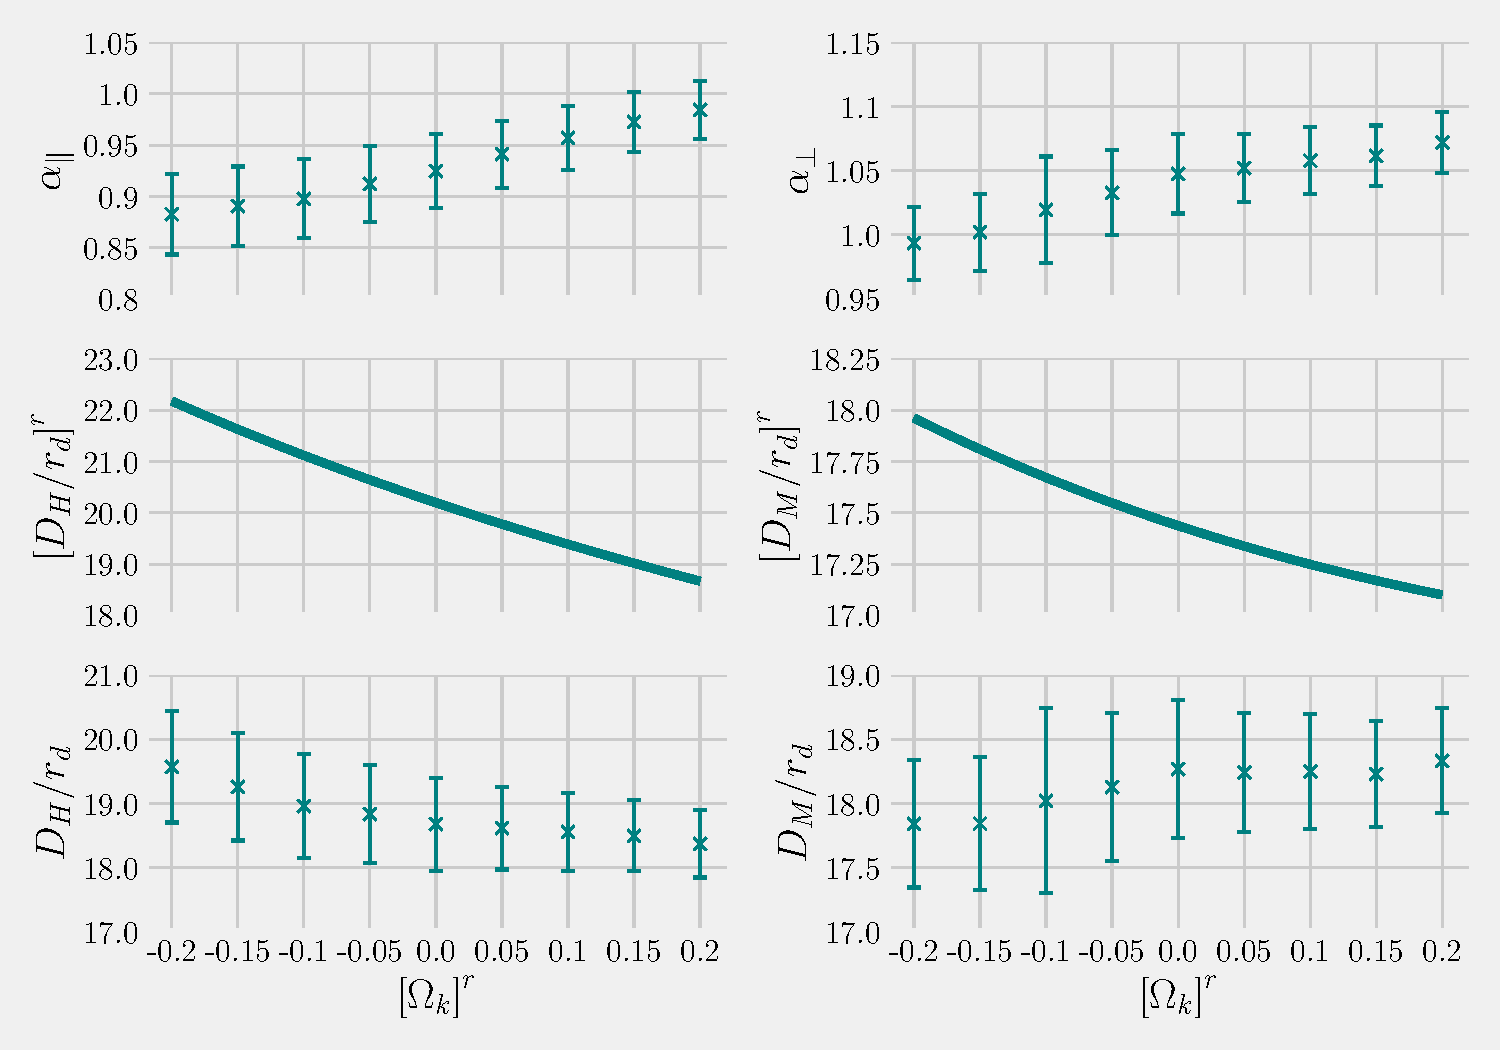
\includegraphics[width=0.8\textwidth]{../figs/phase2_DA_DH_flat.pdf}
		\caption{Derivation of cosmological distance measurements.}
		\label{fig:phase2}
	\end{figure}
	 
\end{frame}

\section{Conclusiones}
\begin{frame}[allowframebreaks]{Conclusiones}

\begin{enumerate}
\item Hemos revisado e implementado la metodología BAO para \textbf{medir} \textbf{distancias} \textbf{cosmológicas} en el Universo, y la hemos aplicado a una muestra de galaxias del cartografiado eBOSS.
\item Hemos usado \textbf{computación} de alto rendimiento para calcular las posiciones de las características BAO de las \textbf{galaxias} \textbf{de} \textbf{eBOSS} junto con sus incertidumbres. 
\item Hemos obtenido unas \textbf{mediciones} \textbf{de} \textbf{distancia} a las galaxias de eBOSS normalizadas a la escala del horizonte de sonido de $D_H/r_d = 18.66 \pm 0.72$ y $D_M/r_d = 18.28 \pm 0.53$.
\item Nuestro resultado principal es que \textbf{no} \textbf{hay} \textbf{dependencia} \textbf{significativa} de estas observables con respecto a cambios en el valor asumido del parámetro de curvatura $ \Omega_k$ en el rango de estudio.
\end{enumerate}
%Por lo tanto, concluimos que la suposición de un valor particular de $\Omega_k$ en la conversión de corrimiento al rojo a distancia no tiene ningún efecto significativo (al menos en el rango $\Omega_k \in [-0.20, +0.20]$) en las distancias cosmológicas inferidas a las galaxias de eBOSS utilizando la metodología BAO.

\end{frame}





%\section{Information processing  issues}
%-----------------------------------------------
%\begin{frame}
%\frametitle{Information processing issues}
%\begin{itemize} 
%\item In collaborative processing
%\begin{itemize}
%\item Target detection, localization, communication, storage, querying...
%\end{itemize}
%\color{lightgray}
%\item  In networking
%\begin{itemize}
%\color{lightgray}
%\item  aggregation, routing, Data naming,...
%\end{itemize}
%\end{itemize}
%\end{frame}
%-----------------------------------------------
%\begin{frame}[fragile] % Need to use the fragile option when verbatim is used in the slide
%\frametitle{Citation}
%An example of the \verb|\cite| command to cite within the presentation:\\~
%Citation \cite{Souza} requires .
%\end{frame}
%%------------------------------------------------
%\section{References}
%\begin{frame}[allowframebreaks]
%\frametitle{References}
% \nocite{*}
% \bibliographystyle{unsrt}
%\bibliography{References}
%\end{frame}

%-----------------------------------------------------------------------------------------
%\section{Acknowledgement}
%\begin{frame} [allowframebreaks]
%\frametitle{Acknowledgement}
%\lipsum[1]
%
%
%\end{frame}
%%-----------------------------------------------------------------------------------------
%
%\begin{frame}
%\Huge{\centerline{Thank You}}
%\end{frame}

%----------------------------------------------------------------------------------------

\begin{frame}
\titlepage % Print the title page as the first slide
\end{frame}

\begin{frame}

\begin{figure}[t]
	\centering
	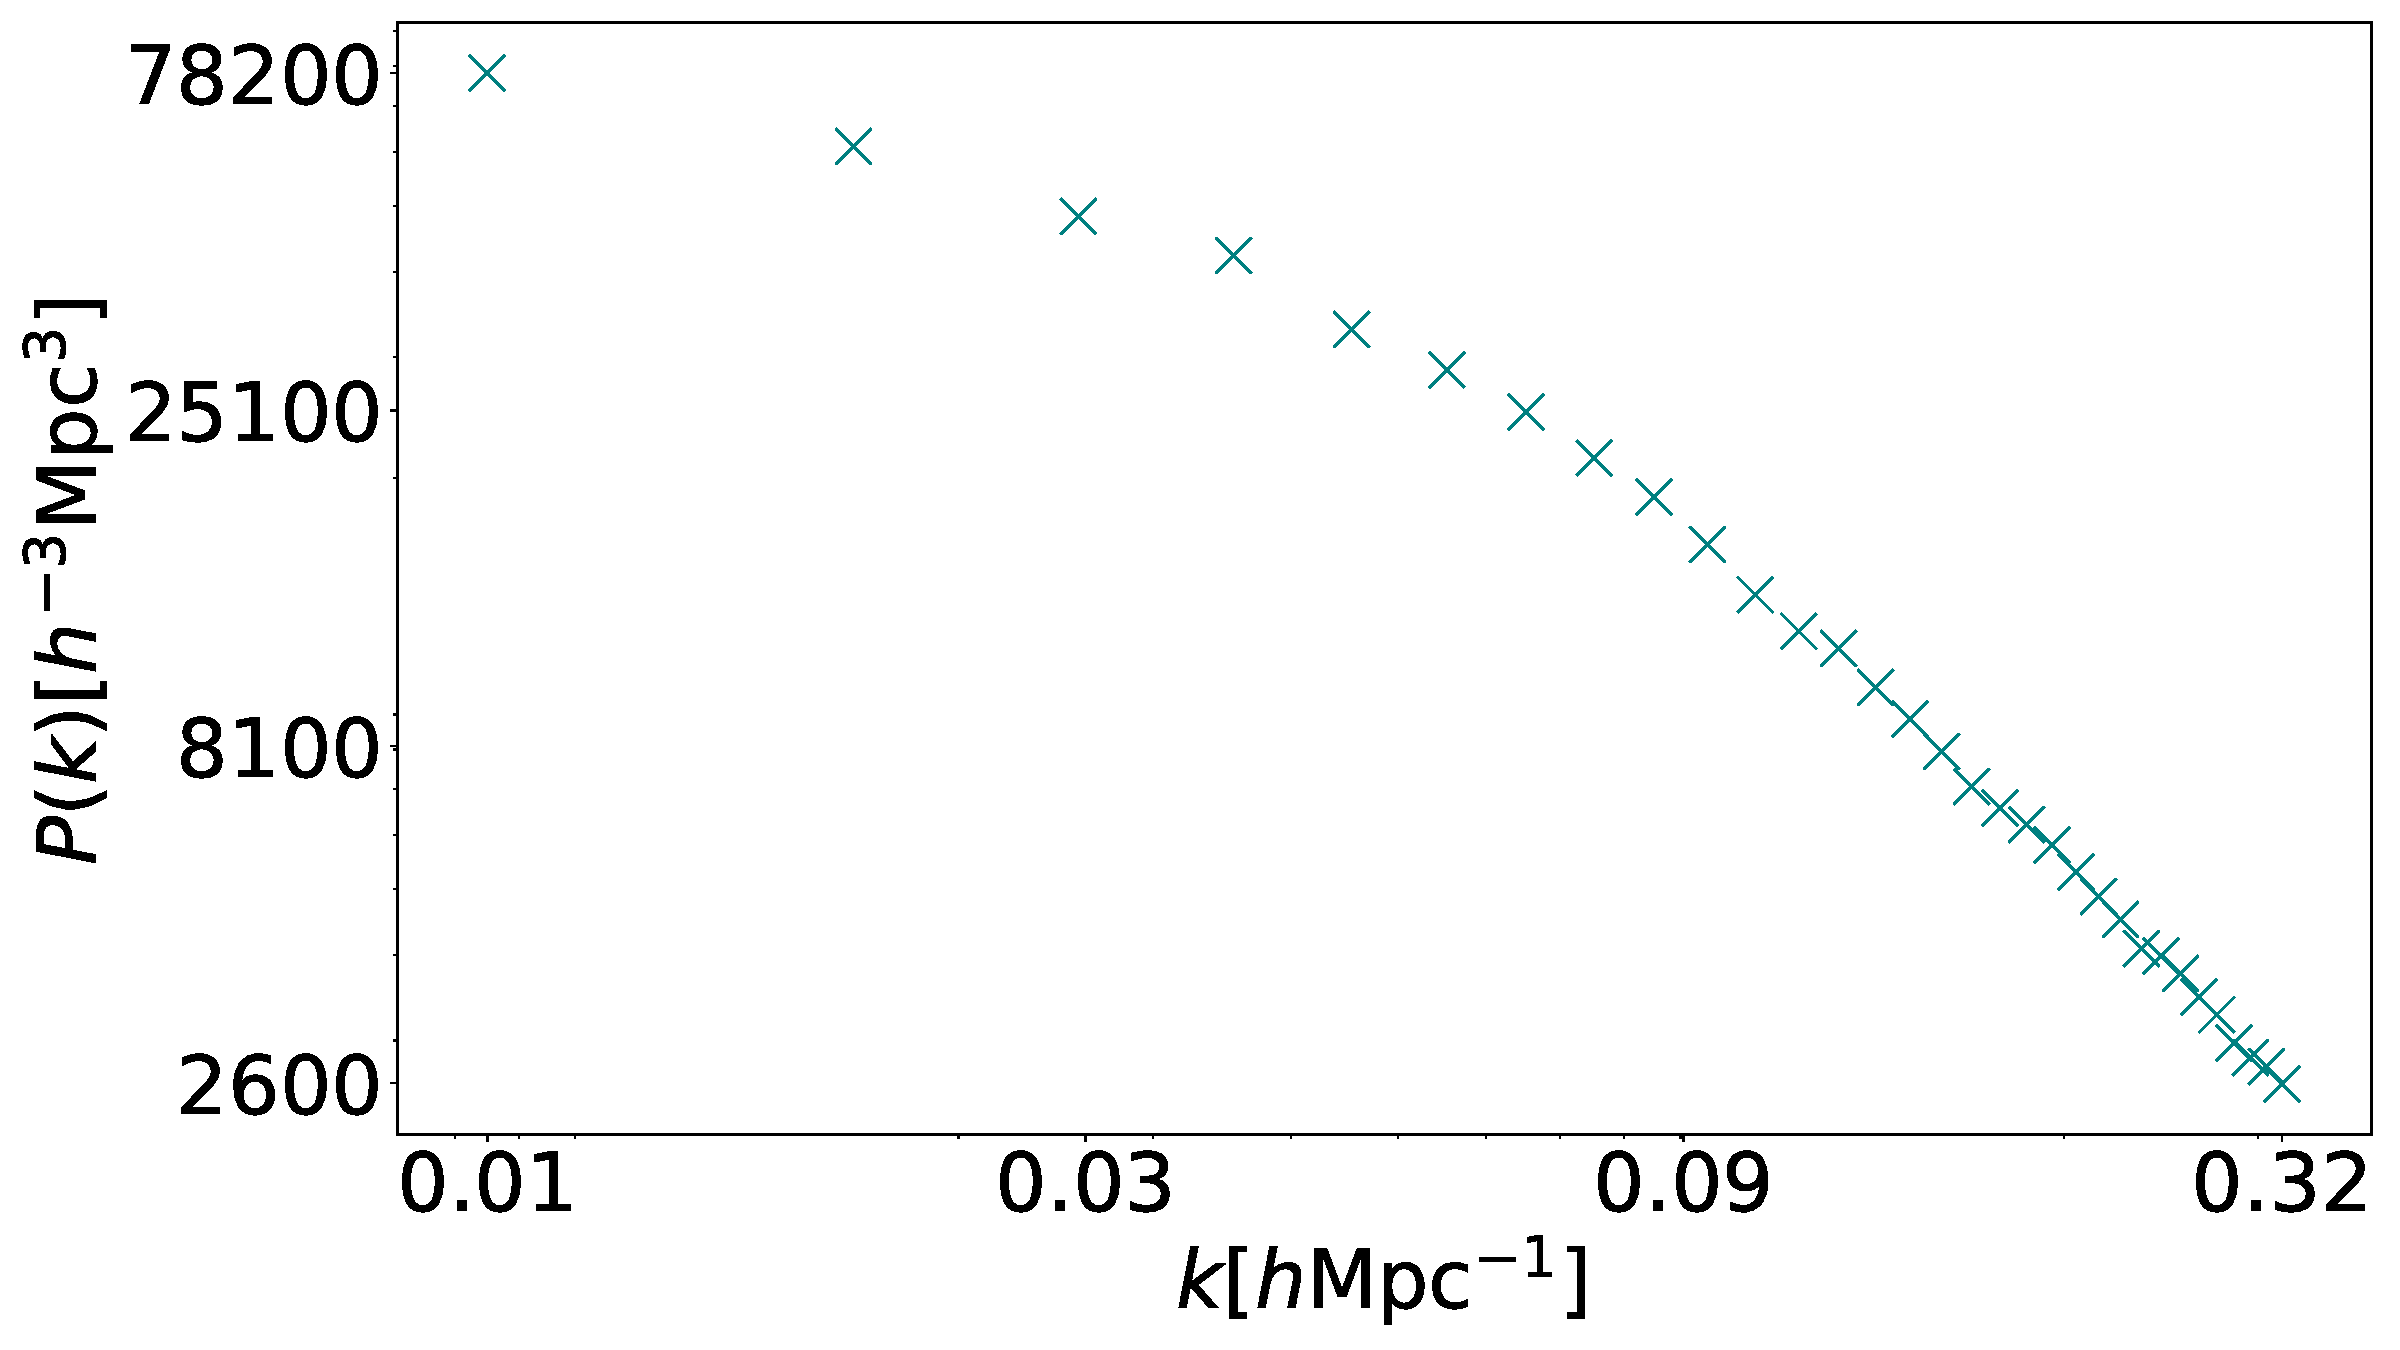
\includegraphics[width=0.8\textwidth]{../figs/Pkrustico.pdf}
	\caption[]{Power spectrum of the LRG eBOSS galaxies.}
	\label{fig:rustico}
\end{figure}
	
\end{frame}
\begin{frame}

\begin{figure}[t]
	\centering
	\subfigure{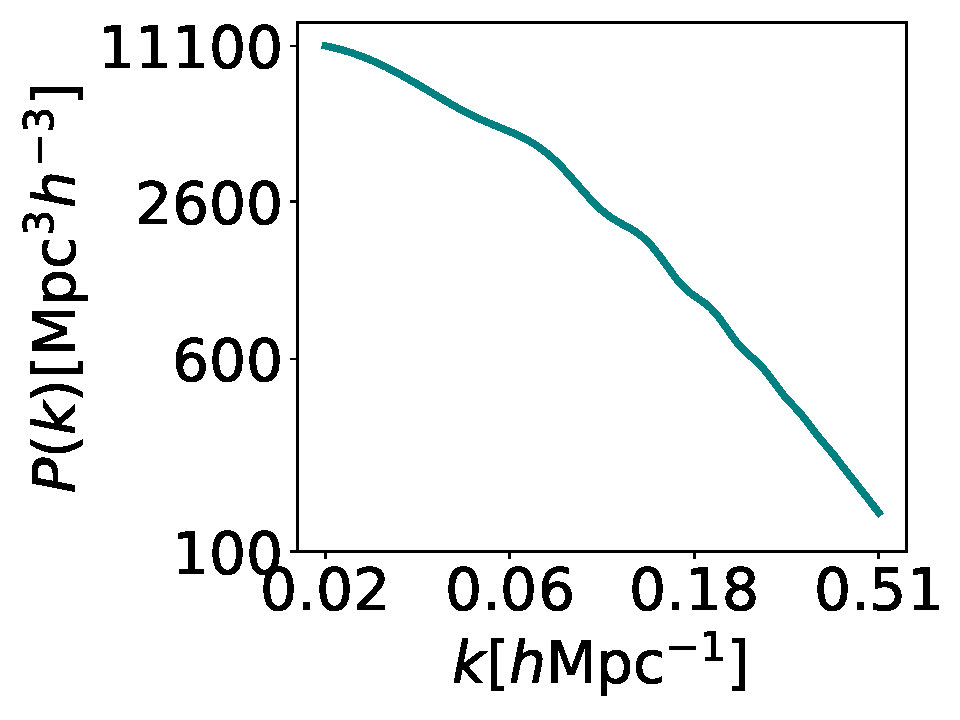
\includegraphics[width=0.32\textwidth]{../figs/Pklin.pdf}}
	\subfigure{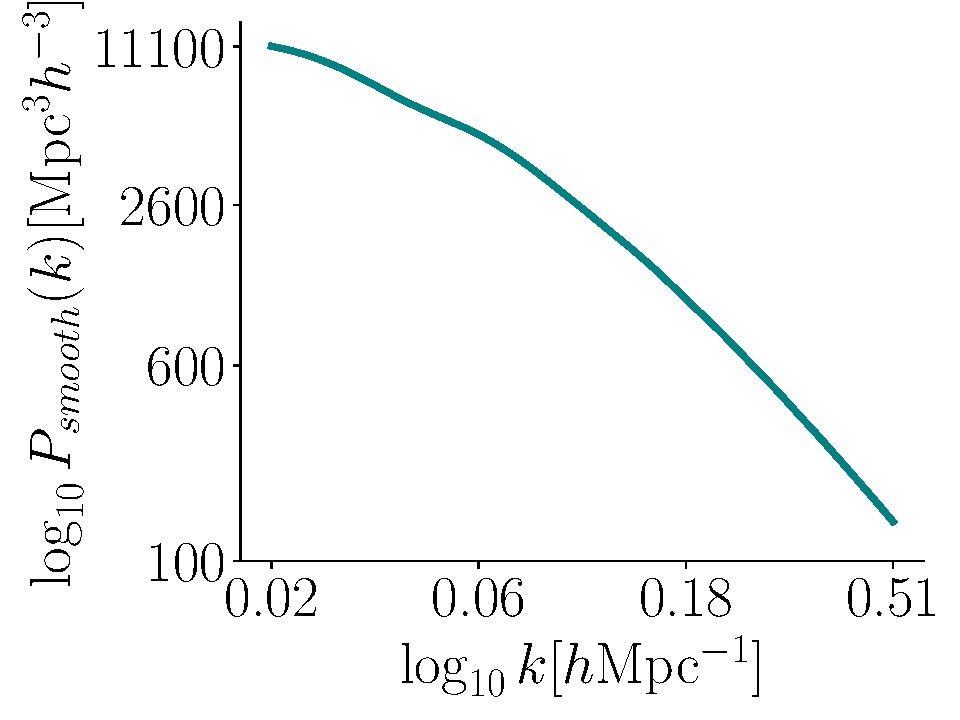
\includegraphics[width=0.32\textwidth]{../figs/Psm.pdf}}
	\subfigure{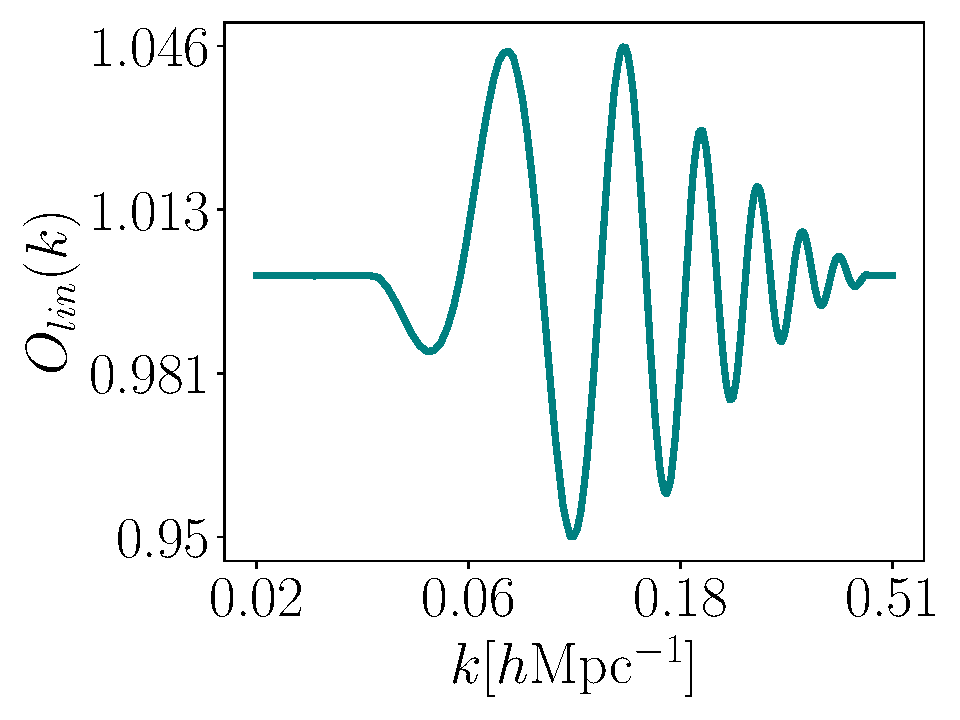
\includegraphics[width=0.32\textwidth]{../figs/Olin.pdf}}
	\caption[]{The template power spectrum and its smooth and the pure BAO components.}
\end{figure}
\end{frame}
\end{document}
